\chapter{Performance evaluation of the relay mode}

As mentioned in chapter \ref{chap:relayproto}, the implementation of the relay protocol on the Waspmote Pro was affected by the heavy limitations of the platform, however functional version of a subset of the specification has been successfully achieved. 

In the same way as described in \ref{sec:ruraltest} a set of experiments has been designed and conducted, with the aim to evaluate the performance enhancements of the proposed two-hop solution in comparison to the standard one-hop LoRaWAN architecture.


\section{Design of test set}

The main goal of this series of experiments is to compare the newly designed two-hop solution with the standard LoRaWAN one-hop communication scheme. The parameters of the experiments were chosen as follows:

\begin{itemize}
\item \emph{Spreading Factor}: SF7 and SF10 were chosen with the aim to test both the fastest available data rate, and a more conservative data rate which leads to a smaller packet error rate. 

\item \emph{Transmission power}: in order to explore the impact of the reduction of transmission power on the packet error rate, it has been decided to test the maximum available power, i.e. 14 dBm, and the minimum one it was known from previous results to receive something at that distance, i.e. 8 dBm;

\item \emph{Payload length}: as seen in single-hop test, packet length may have a great impact on packet error rate, so it has been decided to repeat the experiments with two different payload length (10 and 50 bytes).

\item \emph{Distance from relay}: as described in chapter \ref{chap:relayproto}, one of the goals of implementing a two-hop solution in LoRaWAN networks was to drastically increase the link reliability in condition of high packet error rate. To this aim it has been decided to place the relay node at the maximum possible distance with small packet error rate, which in previous experiments it was discovered to be 1.5 Km from the gateway. 

Given that the maximum distance tested during single-hop experiments was 2.5 Km, it has been decided to start the experiments placing the end-device at 1.0 Km from the relay in order to obtain the same total distance. Than the end-device was placed at 1.5 Km from the relay, that is 3.0 Km from the gateway.
\end{itemize}
The gateway was placed on the terrace of the department of information engineering at the University of Pisa (figure \ref{fig:maprelay}), located in Via Caruso 16, Pisa, Italy. The end-devices and the relay were placed in different spots (figure \ref{fig:maprelay}) along a road inside the natural park of San Rossore, Pisa (Italy). Table \ref{tab:relay_test} summarizes the parameters chosen for this test.

\begin{figure}[]
\centering
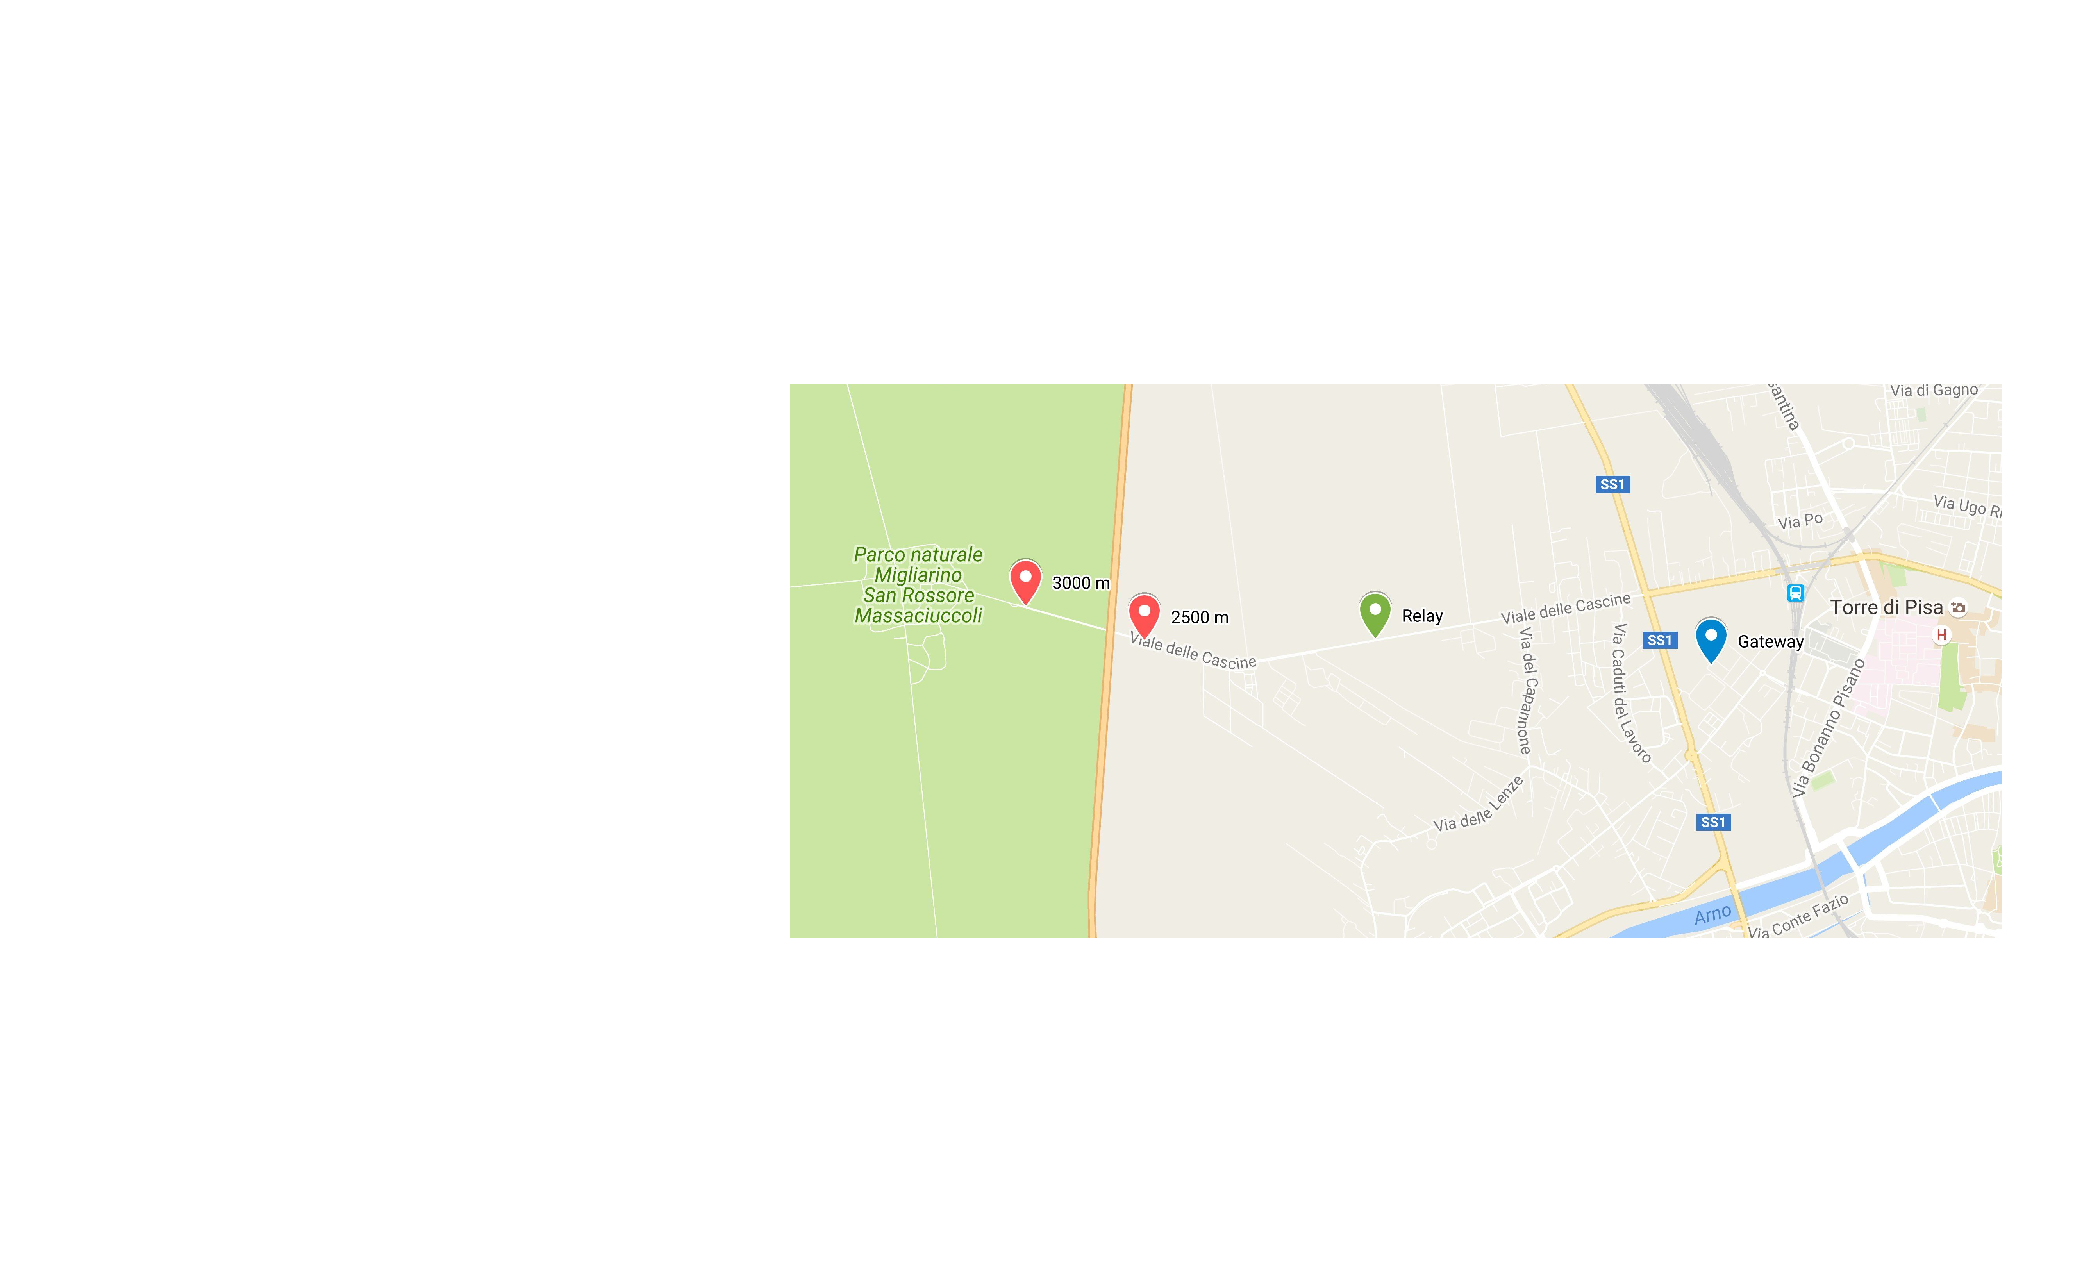
\includegraphics[width=\textwidth]{img/map_relay}
\caption{Map of rural experiments with relay}
\label{fig:maprelay}
\end{figure}

% Please add the following required packages to your document preamble:
% \usepackage{booktabs}
\begin{table}[]
\centering
\caption{Test configurations}
\label{tab:relay_test}
\begin{tabular}{@{}lll@{}}
\toprule
Parameter           & Values & Unit  \\ \midrule
Spreading factor    & 7, 10  &       \\
Transmission power  & 14, 8  & dBm   \\
Payload length      & 10, 50 & bytes \\
Distance from relay & 1, 1.5 & Km    \\ \bottomrule
\end{tabular}
\end{table}

\section{Results}
The results of the experiments, in general, were encouraging, since at 2500 meters from the gateway it was achieved a very low packet error rate combined to the reduction of transmission power, which essentially was the purpose of developing the relay-based solution.

The other great results has been effectively enlarging the coverage area without compromising neither the number of correctly received packets, nor the data rate. In this section the results of the experiments are shown, organized by spreading factor.

\subsubsection{Spreading Factor 7}

SF 7 is, at the same time, the fastest and the less reliable data rate, so it is expected to be the lower bound on the number of correctly received packets. As shown in figure \ref{fig:sf7relay} at 2.5 km all configuration has a percentage of correctly received packets greater then 80\%,  which is a giant leap ahead from the nearly 0\% packets received at the same distance with the single hop scheme. The good performace are confirmed also at 3.0 Km, which was not tested in single-hop scheme, with almost 60\% of correctly received packets in the worst case. In table \ref{tab:cisf7relay} are reported the confidence intervals for each configuration.

\begin{figure}[]
\centering
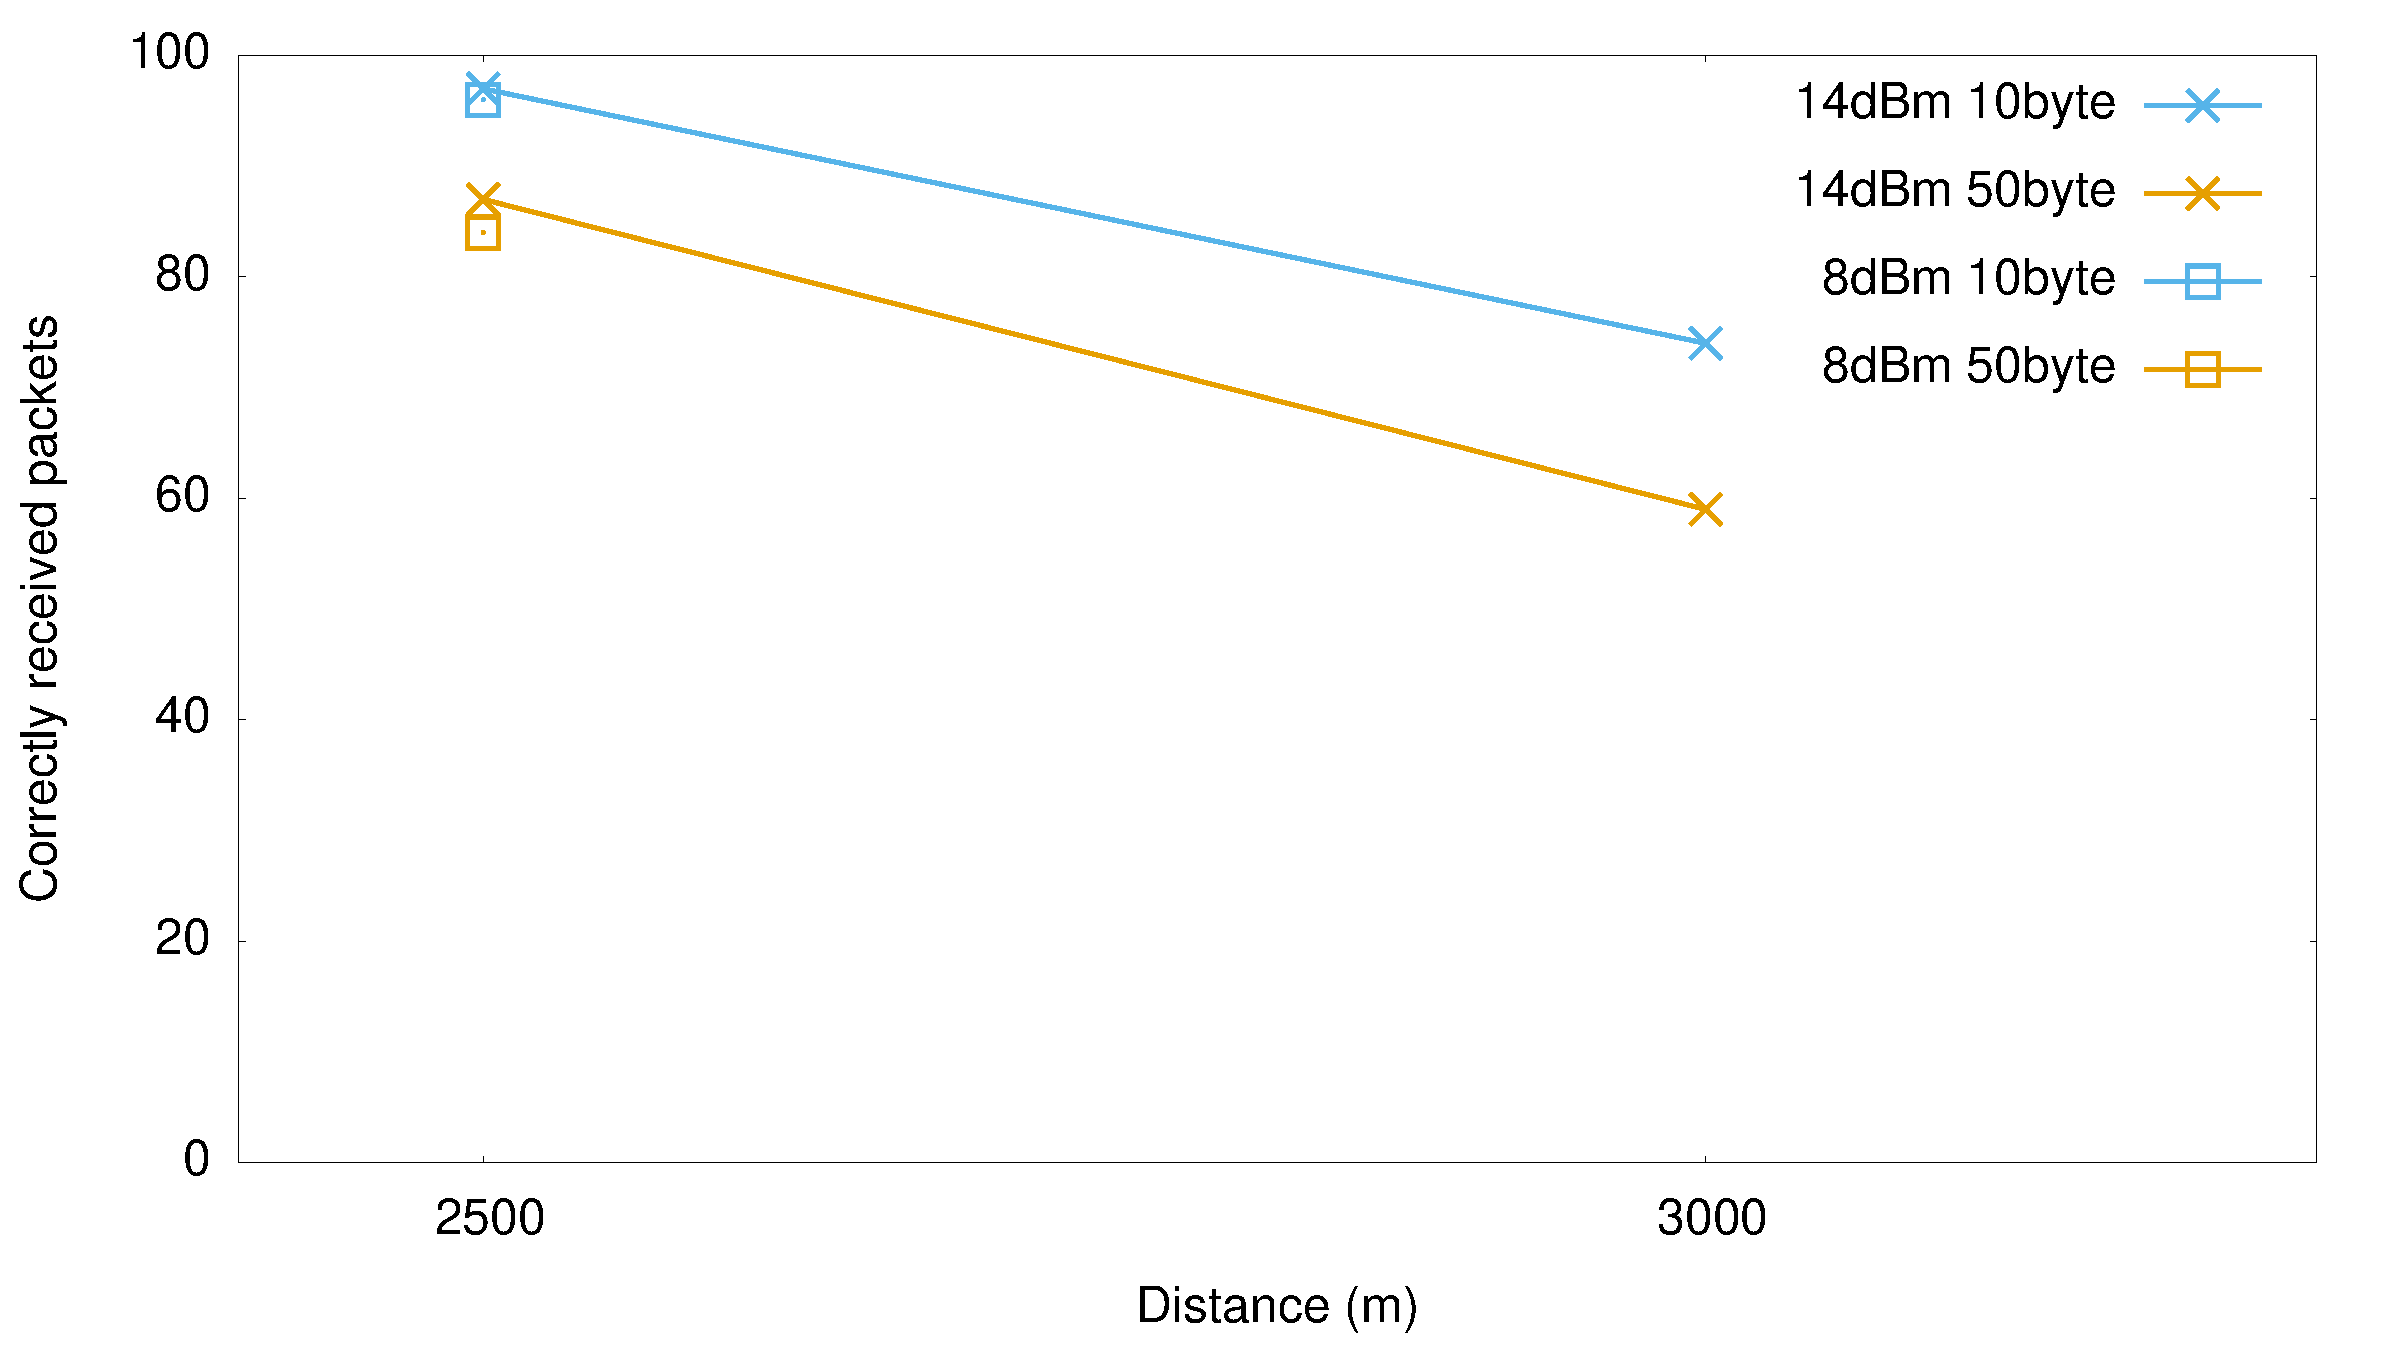
\includegraphics[width=\textwidth]{img/test/relay/sf7}
\caption{Results of two-hop experiments at SF 7}
\label{fig:sf7relay}
\end{figure}


\subsubsection{Spreading Factor 10}
SF 10 was expected to be more reliable, and in fact the results in figure \ref{fig:sf10relay} show even better performances than SF 7. At this data rate is possible to obtain up to 97\% of correctly received packets when considering 8 dBm as transmission power and 10 bytes as payload length.

Therefore this can be considered a remarkable achievement since the new two hop solution decreases both the packet error rate and the needed transmission power with basically no extra infrastructure needed. In table \ref{tab:cisf10relay} are reported the confidence intervals for each configuration. 

\begin{figure}[]
\centering
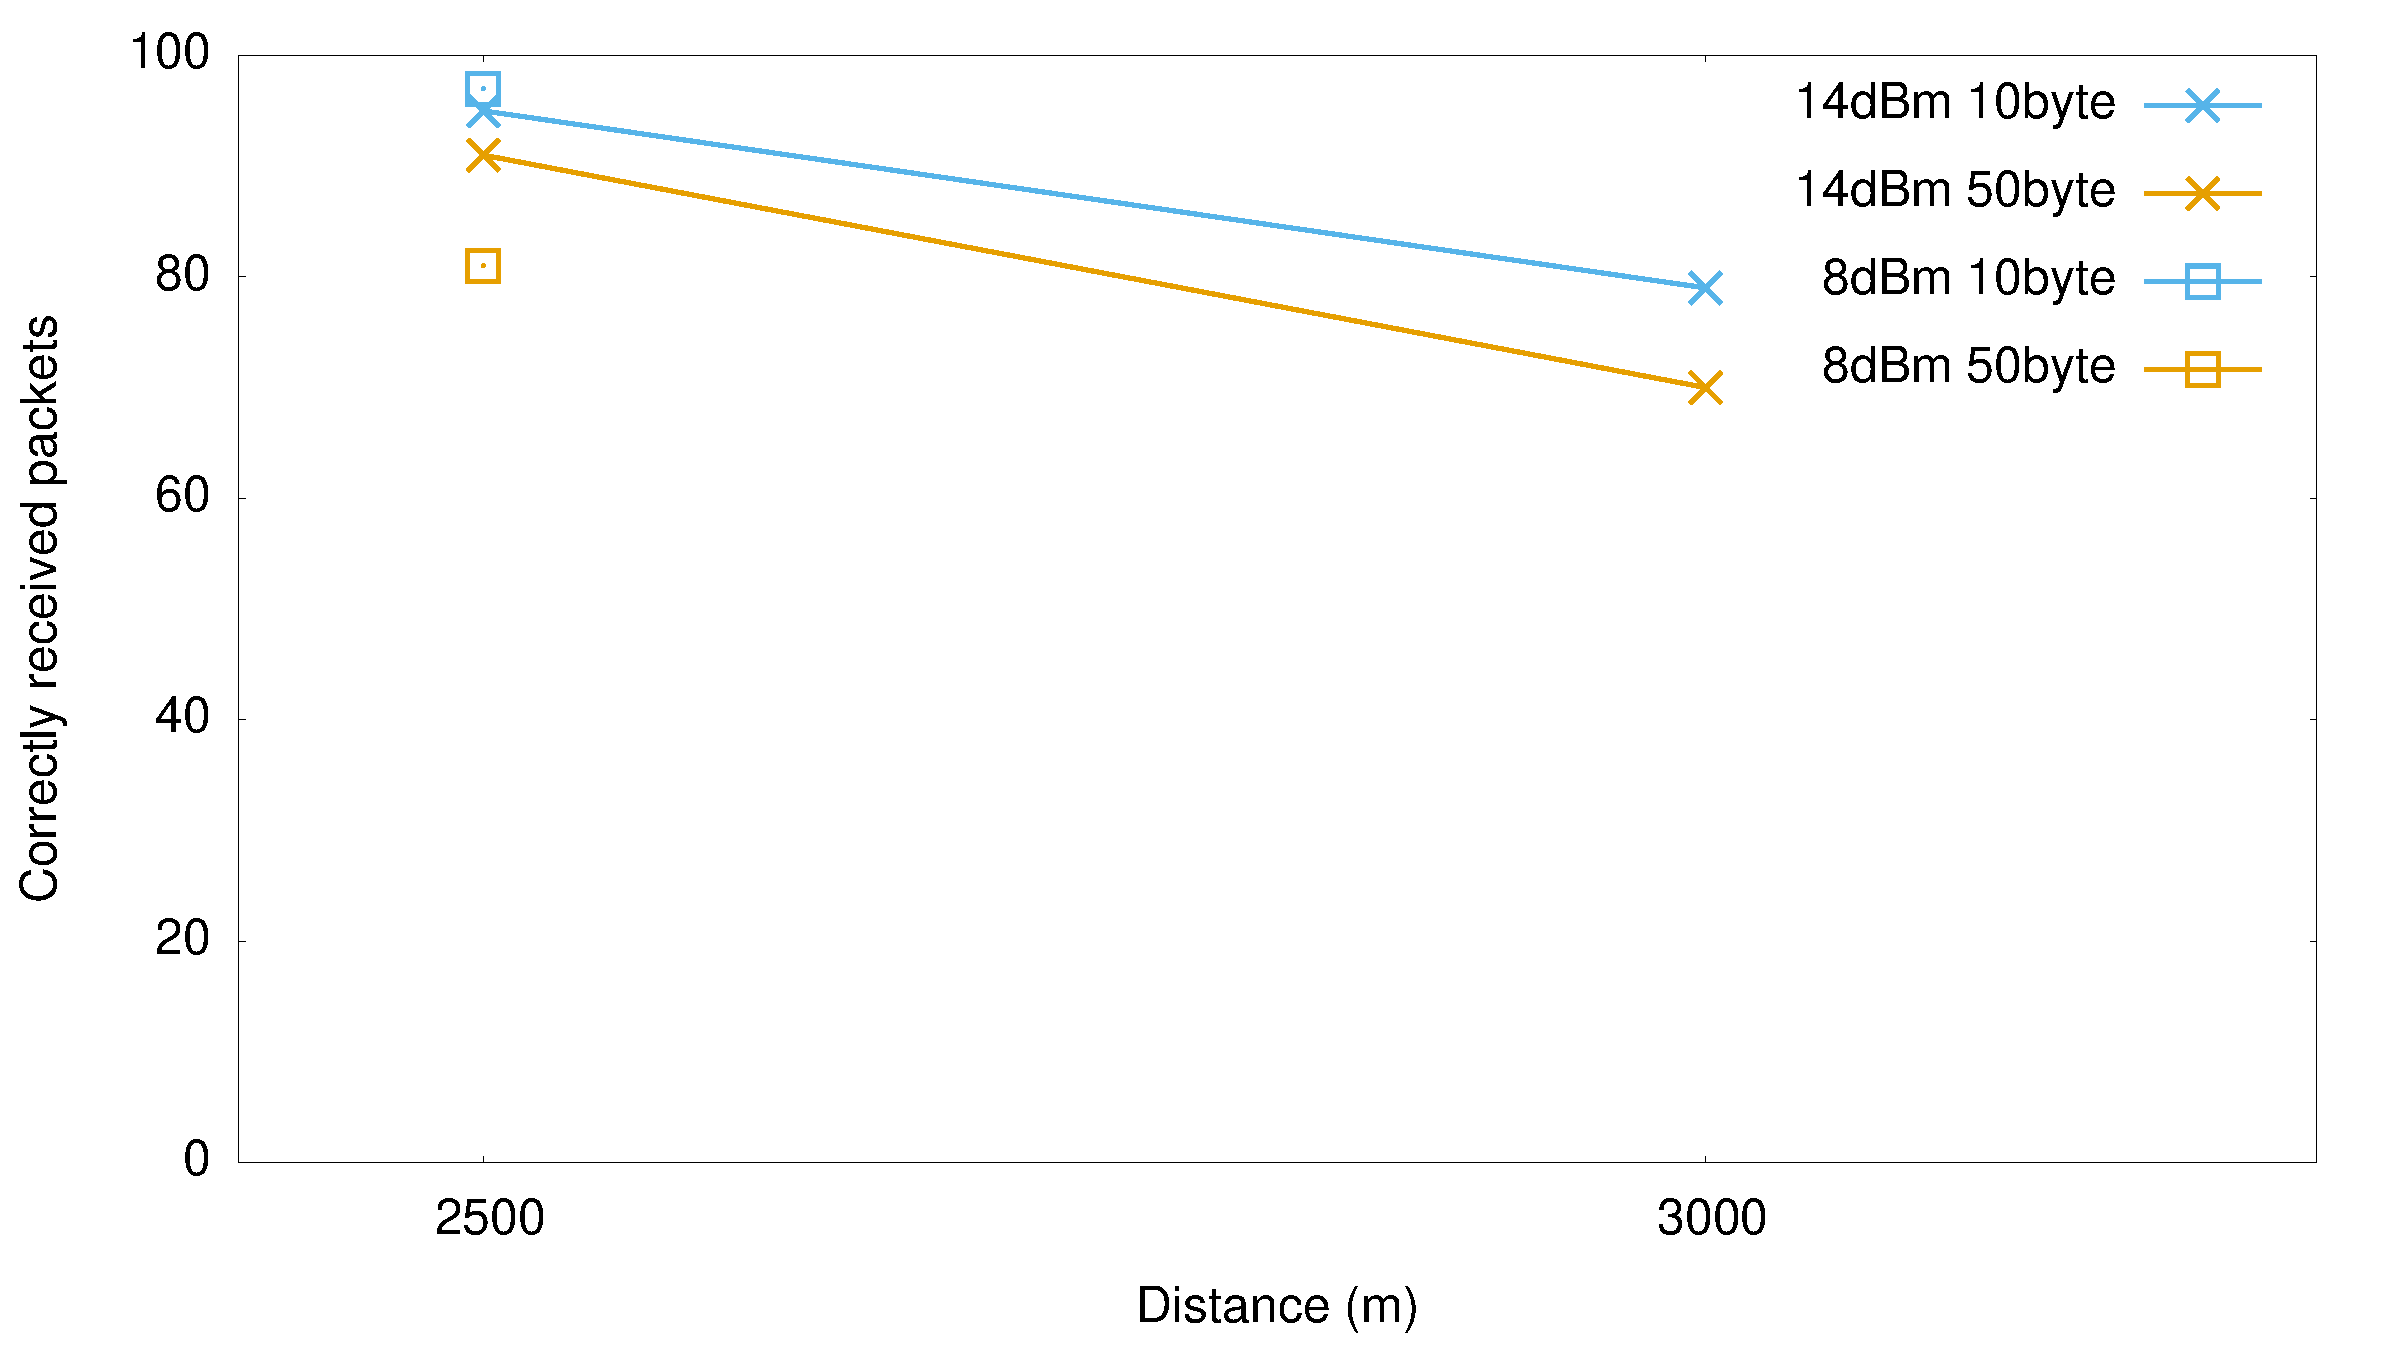
\includegraphics[width=\textwidth]{img/test/relay/sf10}
\caption{Results of two-hop experiments at SF 10}
\label{fig:sf10relay}
\end{figure}



